\documentclass[a4paper,12pt]{article}

%package Start
\usepackage{graphicx}
\usepackage{titling}
\usepackage{color}
\usepackage{listings}
\usepackage[pdftex,dvipsnames]{xcolor}
\usepackage{nomencl}
\usepackage[graphicx]{realboxes}
\usepackage{rotating}
\definecolor{light-gray}{gray}{0.80}
\usepackage{url}
\usepackage[tight,footnotesize]{subfigure}  
\usepackage[top=2cm, bottom=2cm, left=4cm, right=2cm]{geometry}
\usepackage[colorinlistoftodos,prependcaption,textsize=tiny]{todonotes}
\usepackage{titlesec}
%\usepackage{minted} %for js code
\usepackage{tikz}
\usetikzlibrary{arrows,shapes,positioning,shadows,trees}
\usepackage{enumitem}

% start of subsubsubsection environment % %
\titleclass{\subsubsubsection}{straight}[\subsection]

\newcounter{subsubsubsection}[subsubsection]
\renewcommand\thesubsubsubsection{\thesubsubsection.\arabic{subsubsubsection}}
\renewcommand\theparagraph{\thesubsubsubsection.\arabic{paragraph}} % optional; useful if paragraphs are to be numbered

\titleformat{\subsubsubsection}
{\normalfont\normalsize\bfseries}{\thesubsubsubsection}{1em}{}
\titlespacing*{\subsubsubsection}
{0pt}{3.25ex plus 1ex minus .2ex}{1.5ex plus .2ex}

\makeatletter
\renewcommand\paragraph{\@startsection{paragraph}{5}{\z@}%
	{3.25ex \@plus1ex \@minus.2ex}%
	{-1em}%
	{\normalfont\normalsize\bfseries}}
\renewcommand\subparagraph{\@startsection{subparagraph}{6}{\parindent}%
	{3.25ex \@plus1ex \@minus .2ex}%
	{-1em}%
	{\normalfont\normalsize\bfseries}}
\def\toclevel@subsubsubsection{4}
\def\toclevel@paragraph{5}
\def\toclevel@paragraph{6}
\def\l@subsubsubsection{\@dottedtocline{4}{7em}{4em}}
\def\l@paragraph{\@dottedtocline{5}{10em}{5em}}
\def\l@subparagraph{\@dottedtocline{6}{14em}{6em}}
\makeatother

\setcounter{secnumdepth}{4}
\setcounter{tocdepth}{4}

\tikzstyle{every node}=[draw=black,thick,anchor=west,font=\small]
\tikzstyle{json}=[draw=green,fill=green!30]
\tikzstyle{attribute}=[draw=none]
\tikzstyle{defi}=[draw=gray,dashed]
\tikzstyle{textnode}=[draw=gray,fill=gray!30]

% end of subsubsubsection environment % %





\let\abbrev\nomenclature
\renewcommand{\nomname}{List of Abbreviations}
\setlength{\nomlabelwidth}{.25\hsize}
\renewcommand{\nomlabel}[1]{#1 \dotfill}
\setlength{\nomitemsep}{-\parsep}
\makenomenclature 
\newcommand{\Abkuerzung}{
	\printnomenclature
	\newpage
}
%package End

\newcommand{\subtitle}[1]{%
	\posttitle{%
		\par\end{center}
	\begin{center}\large#1\end{center}
	\vskip0.5em}%
}


%\begin{titlepage}
%\begin{center}
\title{XML and NoSQL DBMS: Migration and Benchmarking}
\subtitle{
% TODO->add text from author%
}
%\subtitle{Submitted to the Department of Computer and Information Science at the
%University of Konstanz
%}
%{ \huge \bfseries XML and NOSQL DBMS: Migration and Benchmarking \\[0.4cm] }
%\includegraphics[width=0.15\textwidth]{./unisignet-klein}~\\[1cm]
\input{includes/first-page/author}
%\end{center}
%\end{titlepage}
\begin{document}
	\definecolor{darkgray}{gray}{0.35}
\lstnewenvironment{fakeXML}[1][]{
\lstset{basicstyle=\footnotesize\sffamily,
linewidth=\linewidth,
breaklines=true, 
%numbers=left,
%stepnumber=1,
%numbersep=10pt,
frame=single,
framerule=1.0pt,
%backgroundcolor=\color{darkgray},
language=HTML,
identifierstyle=\color[rgb]{1,0,0},
emph={intersects}, emphstyle=\color{red},
keywordstyle=\color[rgb]{0,0,1},
commentstyle=\color[rgb]{0.133,0.545,0.133},
stringstyle=\color[rgb]{0.627,0.126,0.941},
morekeywords={xml, ref, xs, version, targetNamespace, minOccurs, maxOccurs}
}\lstset{#1}}{}

\lstnewenvironment{fakeJSON}[1][]{
	\lstset{
		basicstyle=\footnotesize\sffamily,
		keywords={typeof, new, true, false, catch, function, return, null, catch, switch, var, if, in, while, do, else, case, break},
		ndkeywords={class, export, boolean, throw, implements, import, this},
		sensitive=false,
		comment=[l]{//},
		morecomment=[s]{/*}{*/},
		morestring=[b]',
		morestring=[b]"
		linewidth=\linewidth,
		breaklines=true,
		escapeinside={\%*}{*)}
		numbers=left,
		stepnumber=1,
		numbersep=10pt,
		frame=single,
		framerule=1.0pt,
		language=JSON,
		emph={}
	}\lstset{#1}}{}

\colorlet{punct}{red!60!black}
\definecolor{delim}{RGB}{20,105,176}
\colorlet{numb}{magenta!60!black}

\lstdefinelanguage{json}{
	basicstyle=\normalfont\ttfamily,
	linewidth=\linewidth,
	numbers=left,
	numberstyle=\scriptsize,
	stepnumber=1,
	numbersep=8pt,
	showstringspaces=false,
	breaklines=true,
	frame=lines,
	literate=
	*{0}{{{\color{numb}0}}}{1}
	{1}{{{\color{numb}1}}}{1}
	{2}{{{\color{numb}2}}}{1}
	{3}{{{\color{numb}3}}}{1}
	{4}{{{\color{numb}4}}}{1}
	{5}{{{\color{numb}5}}}{1}
	{6}{{{\color{numb}6}}}{1}
	{7}{{{\color{numb}7}}}{1}
	{8}{{{\color{numb}8}}}{1}
	{9}{{{\color{numb}9}}}{1}
	{:}{{{\color{punct}{:}}}}{1}
	{,}{{{\color{punct}{,}}}}{1}
	{\{}{{{\color{delim}{\{}}}}{1}
	{\}}{{{\color{delim}{\}}}}}{1}
	{[}{{{\color{delim}{[}}}}{1}
	{]}{{{\color{delim}{]}}}}{1},
}
\lstdefinelanguage{sJSON}{
	keywords={typeof, new, true, false, catch, function, return, null, catch, switch, var, if, in, while, do, else, case, break},
	ndkeywords={class, export, boolean, throw, implements, import, this},
	sensitive=false,
	comment=[l]{//},
	morecomment=[s]{/*}{*/},
	morestring=[b]',
	morestring=[b]"
}

	\renewcommand{\lstlistingname}{Code} 
	
	
	\maketitle
	\thispagestyle{empty}
	
	\newpage
	\section*{Abstract}
		XML and NoSQL database are two growing field in second generation database system, they share some similarities as well as they have some significant difference. 
		This thesis focus on the  comparative analysis of these two database system based on the Use cases and existing solution, we will discuss the data processing, query pattern and  Information Retrieval(\textit{IR})
		
		............
		...........
		............
	
	%\newpage
	\section*{Zusammenfassung(German Abstract)}
	\input{includes/1/abstract-de}
	%\newpage
	\section*{Acknowledgments}
	The completion of this master thesis would not have been possible without the support of many people.
	\thispagestyle{empty}
	\newpage
	\tableofcontents
	\thispagestyle{empty}
	\newpage
	\section{Introduction}
	\setcounter{page}{1}
	\subsection{Motivation}
		\label{motivation}
			Ten years ago XML~\cite{www/xml} was  \textit{de facto} data exchange format. But in recent years a big transformation has been going on in the world of data exchange. The more light weight, less bandwidth-consuming JSON~\cite{www/json} structure has been emerge as an alternative to the XML. Even though these two format are comparatively different regarding features and functionality  and even though both have their own pros and cons, the rise of JSON as new predominant data exchange format is clearly visible. As a result, new  \textit{NoSQL} database systems came along and proved to be successful and the rate of new research papers in this area also increasing.
			......
			....
	
	\subsection{Contribution}
		%The main contribution of this thesis is that it provide the necessary techniques and algorithms migration of data from XML database to NoSQL databases.  More specifically, It will focus on Document store databases MongoDB, Couchbase and Rethinkdb. To complete this task it is necessary to understand general architecture and data model of each of these database as well and the Information Retrieval(\textit{IR}).
At the second part, conversion of Queries in XML data to individual NoSQL database is also ......

.....

		The main contribution of this thesis is that it provides the necessary techniques and algorithms for migrating data from an XML database to NoSQL databases.  More specifically, it will focus on document store databases like MongoDB, Couchbase and Rethinkdb as NoSQL and BaseX as XML Database. To approach this challenge, it is first necessary to understand the general architecture and data model of each of these databases as well as the way how they are queried.
		.....
		
	\subsection{Scope of Thesis}
	%The translation process use in this thesis from One format to another is based on XMark Dataset.
	.....
	....
	\subsection{Overview}
		This thesis is divided into three main sections. Section~\ref{sec:two} defines the techniques and necessary algorithms to convert XML  to JSON. In Section~\ref{sec:three} we will present the analyzed Systems and scope of work. Section~\ref{sec:four} focuses on the performance tests and comparative analysis of each of the NoSQL databases with BaseX, based on the XMark benchmarking project.
		
		
	\newpage
	\section{Semi-structured data}
	\label{sec:two}
	%\section{Preliminaries}

		%\subsection{Semi-structured data}
		\subsubsection{XML and JSON}
			%JSON documents consists of a number of key-value pair (also called attribute-value pair)
			JSON and XML look conceptually similar as they both text based markup language, which are designed to represent data in human-readable form, exchangeable across multiple platforms and parseable by common programming language. When we look at them first, they appear to be quite similar, with difference only in their syntax. But it turns out that they are fundamentally incompatible, as we will see in the following section~\cite{lee2011jxon}.
			\paragraph{Document node}
			\paragraph{Anonymous values}
			\paragraph{Arrays}
			\paragraph{Identifiers}
			\paragraph{Attributes}
			\paragraph{Namespaces}
		
			\todo{ALSO definition of XML and XSD is needed here}
			\\
			\\
			A JSON document consists of two data structures: 
			\begin{itemize}
					\item Objects, which are numbers of key value pairs 
					\item Arrays, which are an ordered list of values
				content...
			\end{itemize}
			A JSON value can be Object, Array, number, string, \texttt{true}, \texttt{false} and \texttt{null}.
		\subsection{Mapping}
			\subsubsection{Friendly}
			\subsubsection{Unfriendly}
			\subsubsection{Array and Object}
			\subsubsection{Mapping approaches}
			\subsubsection{Summary}
		\subsection{Translation from XML to JSON}
			
		\subsection{XML Database}
			\subsubsection{XML Query Language}
		\subsection{NoSQL database}
			\subsubsection{Key/Value storage}
			\subsection{document oriented database}
		\subsubsection{Querying NoSQL database}
	%\newpage
	%this section have to move to in conclusion and future work
	%\section{Related work}
	\newpage
	\section{System/Environment}
	\label{sec:three}
		\subsection{BaseX}
			%
\begin{fakeXML}[label=kml,caption=A simple KML example representing a Point]
<?xml version="1.0" encoding="UTF-8"?>
<kml xmlns="http://www.opengis.net/kml/2.2">
<document>
<placemark>
  <name>New York City</name>
  <description>New York City</description>
  <point>
    <coordinates>-74.006393,40.714172,0</coordinates>
  </point>
</placemark>
</document>
</kml>
\end{fakeXML} 

\begin{fakeJSON}[label=xml,caption=JSON Data]
\end{fakeJSON} 
\begin{figure}
	\centering
	\includegraphics[width=0.9\textwidth]{img/Plot7}
	\caption{An overview of some important indexing structures developed over years}
	\label{trees}
\end{figure}



\begin{lstlisting}
{
"type": "object",
"properties": {
@Name: {
"type": JSON,
"enum": [Fixed]
}
},
required: [@Name]
}
\end{lstlisting}
\begin{minipage}{.5\textwidth}
	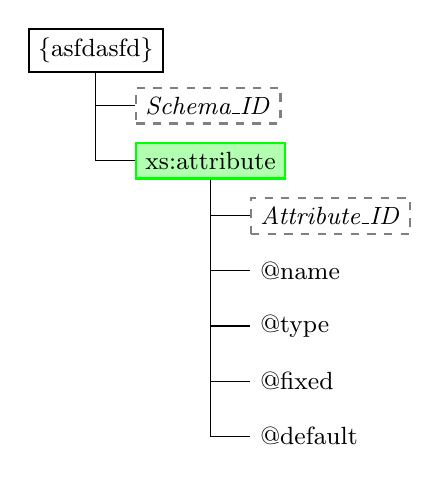
\begin{tikzpicture}[%
	grow via three points={one child at (0.5,-0.7) and
		two children at (0.5,-0.7) and (0.5,-1.4)},
	edge from parent path={(\tikzparentnode.south) |- (\tikzchildnode.west)}]
	\node {\{asfdasfd\}}
	child { node [defi] {\textit{Schema\_ID}}}
	child { node [json] {xs:attribute}
		child { node [defi] {\textit{Attribute\_ID}}}
		child { node [attribute] {@name}}
		child { node [attribute] {@type}}
		child { node [attribute] {@fixed}}
		child { node [attribute] {@default}}
	};
	\end{tikzpicture}
\end{minipage}



Mongodb::

Monodbb's collections have a similar and related documents together that helps better indexing ultimately improve in performance. It will not worth to have single collection of whole XMark data as mentioned in \ref{xmark-nosql}. As we shown in Fig.~\ref{fig:xmark-schema}. we create each collection of each substructure in such a way that we will not lose data as well as most representation of xmark data. All sub-structures \textit{items}, \textit{people}, \textit{open\_auctions}, \textit{closed\_auctions}, \textit{catgraph} and \textit{categories} will be collections which store first group entities of XMark mentioned in data~\ref{xmark-dataset} \texttt{item}, \texttt{person},\texttt{open\_auction}, \texttt{closed\_auction} and \texttt{category} as individual documents respectively. In each of these document, one special field \textbf{doctype} is added to represent the value of the parent. for example, in case of person collection \textit{doctype} will be \textit{people}. This key value set will be also the part of document as shoown in Figure~\ref{code:mongodb-person0}. There is one exceptional case in for \textit{item} collection which has \textbf{regions} as grandparent and name of different regions like asia, europe etc. as parent. because of this reason, the \textit{doctype} for item would look like:
\label{code:xmark-mongo-doctype}
		\subsection{MongoDB}
			%Mongodb is a schemaless document oriented database developed by MongoDB Inc.( then 10gen Inc.) and Open Source Community. It is intended to be flexible data model, fast and Multi-datacenter scalable system written in C++.
\subsubsection{Data Model}
MongoDB uses the concept of \textit{collections} and \textit{documents} to model data. Collection contain any type of documents but generally it has documents with  similar schema. Data has flexible schema where collections do not enforce document to structure rather requirements of our application. A collection is analogous to table of relational database or collection of XML database. Documents are modeled as a data structure following the JSON format which actually store as BSON~\cite{bson}, a binary variant of JSON.  In Mongodb, there are two principle that allow application to represent documents and their relationship: \textit{reference} and \textit{embedded documents}. 
\todo{ need to change following image/json according to xmark data}

\paragraph{Reference}
Reference stores the relationships between data by including links and references from one document to another as in  Figure~\ref{fig:mongodb-ref-doc}. The application can resolve these reference to access the related data\todo{Mongodb data model pg4}
\paragraph{Embedded}
Embedded documents captures relationships between the data by storing related data in a single document structure. The documents in this method are structured as sub-documents\todo{...??} in the in the form of Array or/and Object~\cite{nosql/comparision}. 
\label{mong-xmark-indexing}

\paragraph{Indexing} 
Each document in Mongodb is uniquely identified by a field \textit{\_id} which is a primary index. Hence the collection is sorted by \textit{\_id} by default~\cite{nosql/comparision}.
In addition to primary index, Mongodb supports various user defined indexes for field values of documents including single field index, multikey index, multidimensional index, geo-spatial index, text index and hash index.  Single field, multidimensional and multikey index are organized using B-tree whereas geospatial index is implemented using quad trees.

To index a field that contains a array value, MongoDB provides special indexing called "Multikey". These \textit{multikey} indexes allow MongoDB to return documents from queries using the value of array. 
\begin{figure}
	\centering
	\subfigure[Reference document]{
		\includegraphics[width=0.44\textwidth]{img/mongodb-reference}
		%\caption{R-tree structure}
		\label{fig:mongodb-ref-doc}
	}
	\centering
	\subfigure[Embedded document]{
		\includegraphics[width=0.44\textwidth]{img/mongodb-embedded}
		%\caption{R-tree}
		\label{fig:mongodb-emb-doc}
	}
	\caption{Mongodb document structure}
	\label{fig:mongodb-doc}
	
\end{figure}

\subsubsection{Query Model}
Queries in MongoDB are expressed in a JSON like syntax and send to MongoDB as BSON objects by database drivers\cite{orend2010analysis}. MongoDB's query can be implemented over all documents inside collections, including embedded object and arrays. 
The Query model support following features:
\begin{enumerate}
	\item Queries over documents, embedded subdocuments and arrays
	\item Comparison operators
	\item Conditional Operators
	\item Logical Operators: AND and OR
	\item Sorting 
	\item Group by 
	\item Aggregation per query
\end{enumerate}
In addition to this MongoDB provide a features to for complex aggregation with the use Of MapReduce. The result of MapReduce either can be store as a collection or be removed after result has been return to client\cite{orend2010analysis}.
		\label{couchbase-general}
		\subsection{Couchbase Server}
			% Couchbase Server is NoSQL database that can be used both as a key-value store as well as document store system. As key-value store, it is able to store  multiple data type such as strings, numbers, datetime, and booleans as well as arbitrary binary data. The key-value generally treated as opaque Binary Large Object(BLOB) and don't try to parse it. For document store, data need to be store in the valid JSON format.\todo{
  document database system with flexible data model and easily scalable concept~\cite{cb/brown2013developing}}. Data in Couhbase Server are stored in logical unit called Buckets. Buckets are isolated to each other which also have their own RAM quota and replica settings. These buckets can be technically compare as \texttt{database} in Mongodb or other RDBMS. Couchbase recommends as few as possible number of buckets even it is possible to have up to ten bucket in a single cluster system.These buckets can contains theoretically any type of data. All data type other than JSON can be retrieve only by their key. So it is important to check meta type of data stored in a single document before retrieval. 
%In contrast to Mongodb, Couchbase Server don't have concept of collection, documents are separated by the their \texttt{type}.
\paragraph{Metadata}
For every value stored in database, Couchbase Server generate meta information that is associated with the document~\cite{cb/ostrovsky2014pro}. 
	\subparagraph{Expiration}
		The Time to Live(TTL) also named expiration time is the life time of the document. By default it is 0 which indicates it will never expire, also can be set as Unix epoch time after which document is removed. e.g. The maximum number of seconds you can specify are the seconds in a month, namely 2592000(30 x 24 x 60 x 60). Couchbase Server will remove the item after given number of second it stores. 
	\subparagraph{Check-and-Set(CAS)}
		The CAS value is 64-bit integer that is updated by server when associated item is modified and is a method of optimistic locking~\cite{halici1991optimistic}. It enables to update information only if unique identifier matches the identifier of the document that need to be update. CAS is used to manage concurrency when multiple client attempts to update the same document simultaneously. 
	\subparagraph{Flags} 
		Flags are  as 32 bit integer and are set of SDK specific use for SDK specific need. For example, format in which data is serialize or data type of the object being stored. 
	\\ 
	\\
In addition of expiration, CAS and flags, three other meta store at the time of document creation, \texttt{Id}, the document's key is saved as part of metadata. \texttt{type} is the type of document whether it is JSON for all valid JSON documents and \texttt{Base64} for all other than JSON type is being saved as Base64 encoded string.
\paragraph{Document key}
Every value in Couchbase Server has simple or complex \todo{explain simple or complex}  unique key. unlink Mongodb CB don't generate key automatically, it is up to the application creating the data to supply a unique string value up to 250 characters as key for each document~\ref{cb/ostrovsky2014pro}.
%In case of XMark data each \texttt{id} attributes of  \texttt{item}, \texttt{person}, \texttt{open\_auction}, \texttt{category} represent as key. In case of  \texttt{closed\_auction} and  \texttt{edge} key can be manually generated. 
\paragraph{Document design}

\paragraph{Bucket and vBucket}
		\subsection{Rethinkdb}		
			%RethinkDB~\cite{rethindb} is distributed database system to store  JSON documents that uses efficient query languages named ReQL which automatically parallelize queries in multiple machines. ReQL is based on three main principle: it is completely embedded with programming language, ReQL queries can be passed as pipeline from one stage to another to get required result that means it is possible to use series of simple queries together to perform complex operation. Finally, all the queries are executed in server without any intermediate network round trip required the server and clients. 
		\subsection{Summary}
	\newpage
	\section{Performance/Experiments}
	\label{sec:four}
		\subsection{XMark}
		\label{xmark}
			The XML benchmarking project XMARK~\cite{xmark/original} is one of the most popular and most commonly used XML benchmarking project to date. It provides a small executable tool called \textit{xmlgen} that allows for the creation of a synthetic XML dataset based on a fixed schema describing an Internet auctions database. Its generator can be used to build  a single record with a large, hierarchic XML tree structure. A factor can be specified to scale the generated data, ranging from a few kilobytes to any arbitrary size limited by the capacity of the system. The textual part of resulting XML document is constructed from 17,000 most frequently occurring words of Shakespeare's plays.
\label{xmark-dataset}
\subsubsection{Dataset}
The main entities of XMark data come with two group. In first group \texttt{person},\texttt{open\_auction}, \texttt{closed\_auction}, \texttt{item} and \texttt{category} are expressed through the reference as in Fig.~\ref{fig:xmark-reference} whereas second group entities \texttt{annotation} and \texttt{description} take after the natural language text and are document-centric element structure. \texttt{annotation} and \texttt{description} are embedded into sub-tree of group one entities. 
\\
As shown in Fig.~\ref{fig:xmark-tree}, \texttt{items} are the objects for sale or already sold. Each \texttt{item} caries a unique identifier and having properties like payment information(credit card, money order), \texttt{description} , a reference to the seller etc., all encoded as element. Each item is assign to world region like \texttt{asia}, \texttt{africa} etc. as a parent of an item. \texttt{open\_auctions} are auctions in progress which contains bid history(increase/decrease over time) with reference to bidder and seller, current bid etc. \texttt{closed\_auctions} are the auctions that are completed, which has reference to buyer, seller and item that is sold, amount of price etc. \texttt{people} are the information about \texttt{person} that are connected to buyer/seller of open\_auctions, closed\_auctions etc. \texttt{categories} are implemented to classify items which has a name and description. A \texttt{catgraph} links categories into a network.  The full semantic of XMark dataset can be found in~\cite{xmark/original}.
	%\input{includes/custom/xmark-tree}

\begin{figure}
	\centering
	\subfigure[Reference in \textit{XMark}]{
		\includegraphics[width=0.40\textwidth]{img/xmark-references.png}{
			\label{fig:xmark-reference}
		}
	}
	\centering
	\subfigure[Reference in \textit{XMark} dataset tree~\cite{xmark/original}]{
		\includegraphics[width=0.40\textwidth]{img/xmark-tree.png}{
			\label{fig:xmark-tree}
		}
	}
	\caption{XMark data tree and reference}
	\label{fig:xmark-tree-reference}
\end{figure}
\begin{figure}
	\centering
	\includegraphics[width=0.90\textwidth]{img/xmark-schema-4}
	\caption{XMark ER-Diagram. Nodes, solid arrows, and dashed arrows represent schema elements (or attributes, with prefix '@'), structural links, and value links, respectively. Elements with suffix '*' are of SetOf type\cite{xmark/schema-sumerize}}
	\label{fig:xmark-schema}
\end{figure}

\todo{figure need to create}

\subsubsection{Queries}
\todo{change the style of queries and complete the queries}
The XMark project contains 20 XQuery Queries~\cite{xmark/original} which focus on various aspect of language such as agrression, reference, ordering, wildcard expressions, joins, user defined functions etc.\cite{xmark/mlynkova2008xml}
\label{xmark-queries}
	\begin{enumerate}[label=Q\arabic*.]
		\item Return the name of the person with ID "person0". \\
		\begin{fakeXML}
			let $auction := doc("xmark.xml") return
			for $b in $auction/site/people/person[@id = "person0"]
			return $b/name/text()
		\end{fakeXML}
		\item Return the initial increases of all open auctions. \\
		\begin{fakeXML}
			let $auction := doc("xmark.xml") return
			for $b in $auction/site/open_auctions/open_auction
			return <increase>{ $b/bidder[1]/increase/text() }</increase>
		\end{fakeXML}
		\item Return the IDs of all open auctions whose current increase is at least twice as high as the initial increase. \\
		\begin{fakeXML}
			let $auction := doc("xmark.xml") return
			for $b in $auction/site/open_auctions/open_auction
			where zero-or-one($b/bidder[1]/increase/text()) * 2 <=
			$b/bidder[last()]/increase/text()
			return <increase first="{$b/bidder[1]/increase/text()}"
			last="{$b/bidder[last()]/increase/text()}"/>
		\end{fakeXML}	
	\end{enumerate}
	.....
		\subsection{Evaluation of Test devices}
		\subsection{XMark data into NoSQL Database}
			\label{xmark-nosql}
			A synthetic XMARK dataset consist of one(huge) record in tree structure~\cite{xmark/VIST}. However, as already mentioned in \ref{xmark}, each subtree in schema, \texttt{items}, \texttt{people}, \texttt{open\_auctions} , \texttt{closed\_auctiosn},\texttt{catgraph} and \texttt{categories} contains large number of instances in the database which are indexed. In most of NoSQL system, this scenario is different, each instance has it's own index structure, the dataset cannot be in just a huge block. As the data model of NoSQL do not match this single structure-encoded sequence, we breakdown it's tree structure into set of sub-structure without losing the overall data and create index for each of them.
Beside this, each NoSQL database has their own data model design, unlike most of the XML databases, which have more similar \todo{???}structure than NoSQL, we need to define model design for each of those databases separately. 
\\
\\
The generalized concept of XMark data to NoSQL database is given here, but it might be slightly  different each of them.
 All sub-structures \textit{items}, \textit{people}, \textit{open\_auctions}, \textit{closed\_auctions}, \textit{catgraph} and \textit{categories} are the basic for document fragmentation which store first group entities of XMark mentioned in ~\ref{xmark-dataset} \texttt{item}, \texttt{person},\texttt{open\_auction}, \texttt{closed\_auction} and \texttt{category} as individual documents respectively. In each of these document, one special field \textbf{type} is added to represent the value of the parent. for example, in case of person collection \textit{type} will be \textit{people}. This key value set will be also the part of document as shown in Code 2\todo{ref:code:nosql-person0}. There is one exceptional case for \textit{items}  which has \textbf{regions} as grandparent and name of different regions like \textit{asia}, \textit{europe} etc. as parent, the \textit{type} will be \textit{"items"} as others and one extra field need to be added to represent each region, so there will be one more field in case of \textit{item}.

 \begin{fakeJSON}[label=json,caption=\textit{doctype} and \textit{regions} for item which has region name \textit{asia}]
 	"type":"items",
 	"regions":"asia"
 \end{fakeJSON}
  
 \label{code:nosql-person0}
\begin{fakeJSON}[label=json,caption=General NoSQL data representation of XMARk data]
	{
		"id": "person0",
		"type": "people",
		"name": "Kasidit Treweek",
		"emailaddress": "mailto:Treweek@cohera.com",
		"phone": "+0 (645) 43954155",
		"homepage": "http://www.cohera.com/~Treweek",
		"creditcard": "9941 9701 2489 4716",
		"profile": {
			"income": 20186.59,
			"interest": [{
				"category": "category251"
			}],
			"education": "Graduate School",
			"business": "No"
		}
	}
\end{fakeJSON} 

\begin{fakeXML}[label=xml,caption=XMARK data with of \textit{person0}]
	
	<person id="person0">
	<name>Kasidit Treweek</name>
	<emailaddress>mailto:Treweek@cohera.com</emailaddress>
	<phone>+0 (645) 43954155</phone>
	<homepage>http://www.cohera.com/~Treweek</homepage>
	<creditcard>9941 9701 2489 4716</creditcard>
	<profile income="20186.59">
	<interest category="category251" />
	<education>Graduate School</education>
	<business>No</business>
	</profile>
	</person>
\end{fakeXML} 

\iffalse
\begin{minipage}{.5\textwidth}
	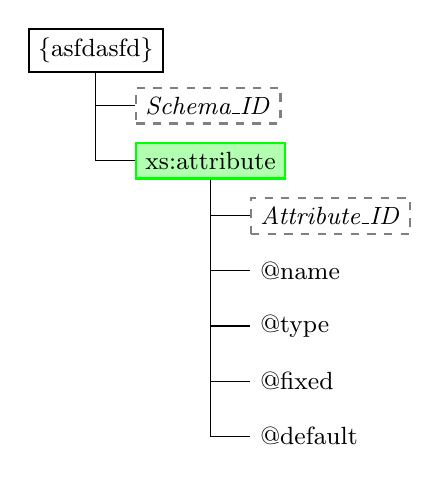
\begin{tikzpicture}[%
	grow via three points={one child at (0.5,-0.7) and
		two children at (0.5,-0.7) and (0.5,-1.4)},
	edge from parent path={(\tikzparentnode.south) |- (\tikzchildnode.west)}]
	\node {\{asfdasfd\}}
	child { node [defi] {\textit{Schema\_ID}}}
	child { node [json] {xs:attribute}
		child { node [defi] {\textit{Attribute\_ID}}}
		child { node [attribute] {@name}}
		child { node [attribute] {@type}}
		child { node [attribute] {@fixed}}
		child { node [attribute] {@default}}
	};
	\end{tikzpicture}
\end{minipage}

\fi
			\newpage			
			\subsubsection{MongoDB}
			\label{xmark-mongodb}
			
% % This section can go on section:4.2
Mongodb uses the concept of \textit{collections} and \textit{documents} to model data. collections are the grouping of documents which generally have similar schemas. Data in Mongodb has flexible schema where collections do not enforce document structure rather requirements of our application. \todo{A collection is analogous to collection in XML database????}.  Documents are modeled as a data structure following the JSON format which is composed of key and value pair. There are two principle that allow application to represent documents and their relationship: \textit{reference} and \textit{embedded documents}. 
\todo{ need to change following image/json according to xmark data}
\begin{figure}
	\centering
	\subfigure[Reference document]{
		\includegraphics[width=0.44\textwidth]{img/mongodb-reference}
		%\caption{R-tree structure}
		\label{fig:mongodb-ref-doc}
	}
	\centering
	\subfigure[Embedded document]{
		\includegraphics[width=0.44\textwidth]{img/mongodb-embedded}
		%\caption{R-tree}
		\label{fig:mongodb-emb-doc}
	}
	\caption{Mongodb document structure}
	\label{fig:mongodb-doc}
	 
\end{figure}

\paragraph{Reference}
	Reference store the relationships between data by including links and references from one document to another as in  Figure~\ref{fig:mongodb-ref-doc}. The application can resolve these reference to access the related data\todo{Mongodb data model pg4}
\paragraph{Embedded}
	Embedded documents captures relationships between the data by storing related data in a single document structure. The documents in this method are structured as sub-documents\todo{...??} in the in the form of Array or/and Object~\cite{nosql/comparision}. 
	
\paragraph{Indexing} 
	Each document in Mongodb is uniquely identified by a field \textit{\_id} which is a primary index. Hence the collection is sorted by \_id by default. \todo{but note that this primary key index is not a clustered index in Database terms. I.e. the index entries only contains pointers to actual documents in the MongoDB data files. Documents are not physically stored in the order of \_id on disks.??  ::expand...page:9}~\cite{nosql/comparision}
	

\subsubsubsection{XMARK in Mongo}

\begin{fakeJSON}[label=json,caption=Mongodb data representation of XMARk data]
	{
		"_id": "person0",
		"doctype": "people",
		"name": "Kasidit Treweek",
		"emailaddress": "mailto:Treweek@cohera.com",
		"phone": "+0 (645) 43954155",
		"homepage": "http://www.cohera.com/~Treweek",
		"creditcard": "9941 9701 2489 4716",
		"profile": {
			"income": 20186.59,
			"interest": [{
				"category": "category251"
			}],
			"education": "Graduate School",
			"business": "No"
		}
		....
	}
\end{fakeJSON} 

\begin{fakeXML}[label=xml,caption=XMARK data with of \textit{person0}]
	
	<person id="person0">
	<name>Kasidit Treweek</name>
	<emailaddress>mailto:Treweek@cohera.com</emailaddress>
	<phone>+0 (645) 43954155</phone>
	<homepage>http://www.cohera.com/~Treweek</homepage>
	<creditcard>9941 9701 2489 4716</creditcard>
	<profile income="20186.59">
	<interest category="category251" />
	<education>Graduate School</education>
	<business>No</business>
	</profile>
	...
	</person>
\end{fakeXML} 

	
\subsubsubsection{Queries}

	
	

			\subsubsection{Couchbase Server}
			\label{xmark-couchbase}
			
\paragraph{Document design}
For Couchbase Server, there is no need to change any structure of XMark NoSQL representation as mentioned in \ref{xmark-nosql} as there is no concept of fragmentation like in \textit{collections} of Mongodb or \textit{tables} in Rethinkdb. The documents are identified by \textit{doctype}. All of these documents are inserted in a single Bucket with \textit{id} as key. For those documents that doesn't have id field, will be manually generated.

\subsubsubsection{Queries}


			\subsubsection{Rethinkdb}
			\label{xmark-rethinkdb}
			RethinkDB~\cite{rethindb} is distributed database system to store  JSON documents that uses efficient query languages named ReQl which automatically parallelize queries in multiple machines. ReQL is based on three main principle: it is completely embedded with programming language, ReQL queries can be passed as pipeline from one stage to another to get required result that means it is possible to use series of simple queries together to perform complex operation. Finally, all the queries are executed in server without any intermediate network round trip required the server and clients. 
\paragraph{Data Model}
The relationships between documents can be can be created by embedded arrays of documents and linking document stores in multiple tables similar to MongoDB in ~\ref{xmark-mongodb}.
Rethinkdb stores JSON documents with binary on disk serialization. RethinkDB implicitly support JSON data types: \texttt{object}, \texttt{array}, \texttt{number}, \texttt{boolean} and \texttt{null}. 
RethinkDB allows embedded JavaScript expressions anywhere as part of query language

\paragraph{Indexing}
At the time of table creation, RethinkDB provide option of specifying the attributes that will serve as primary key, by default \texttt{id}  will serve if primary key attribute is not specified.		
		\subsection{Benchmarking}
		\subsection{Summary}
	\newpage
	\section{Discussion}
	\section{Conclusion}
	\label{conc}
	
	\newpage
	\section{Future Work}
	\label{s.future}
	storing in the memory
	\newpage
	\bibliographystyle{unsrt}
	\bibliography{includes/reference}
	\newpage
	\listoffigures
	\newpage
	\listoftables
	\newpage
	\lstlistoflistings
	%%%%%%%%%%%%%%%%%%%%%abbreviate
	\abbrev{XML}{Extensible Markup Language}
	\abbrev{JSON}{JavaScript Object Notation}
	\abbrev{VM}{Virtual Machine}
	\abbrev{JVM}{Java Virtual Machine}
	\abbrev{IPC}{Inter-process Communication}
	\abbrev{SDK}{Software Development Kit}
	\abbrev{GUI}{Graphical User Interface}
	\abbrev{XML}{Extensible Markup Language}
	\abbrev{HTML}{Hypertext Markup Language}
	\abbrev{DOM}{Document Object Model}
	\abbrev{IR}{Information Retrieval}
	\abbrev{CB}{Couchbase Server}
	
\end{document}	
